% !TeX TS-program = xelatex

\documentclass[compress, 8pt]{beamer}

\usepackage{presentationtemplate}
\usepackage[askip=3mm, bskip=3mm]{terminal}
\usepackage[linenosfontsize=\tiny, askip=3mm, bskip=3mm]{mylisting}
\usepackage{tcolorbox}
\usepackage{tikz}
\usetikzlibrary{positioning}

\newtcolorbox{task}{
    colback=yellow!50!white,
    boxrule=0.02cm,
    colframe=black,
    sharp corners,
    left=0mm,
    right=0mm,
    top=0mm,
    bottom=0mm,
    before upper={\textbf{Задание}:\:},
}

\title{Массивы}

\begin{document}

\frame[plain]{\titlepage}

\begin{frame}[fragile]

    \frametitle{Mассив}

    \textbf{Массивом} (array) в C++ называется последовательность объектов
    одного типа, непрерывно расположенные в памяти один за другим.
    Все элементы массива имеют один и тот же размер.

    \hfill \break
    Каждому элементу массива ставится в соответствие \textbf{индекс}.
    Первому элементу массива соответствует индекс \verb|0|, второму ---
    \verb|1| и т.д.

    \hfill \break
    \hfill \break
    \centering
    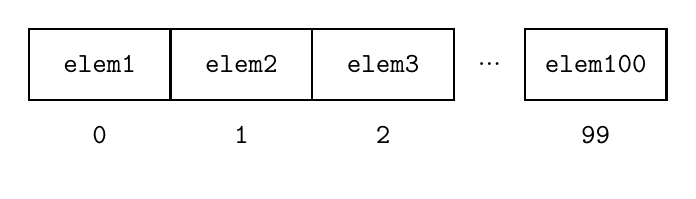
\begin{tikzpicture}[
        cell/.style={
            rectangle,
            thick,
            minimum width=18mm,
            minimum height=9mm
        }
    ]
        \node[cell, draw]               (elem1)                                      {\verb|elem1|};
        \node[cell, draw]               (elem2)   [right=-\pgflinewidth of elem1] {\verb|elem2|};
        \node[cell, draw]               (elem3)   [right=-\pgflinewidth of elem2] {\verb|elem3|};
        \node[cell, minimum width=9mm]  (break)   [right=-\pgflinewidth of elem3] {...};
        \node[cell, draw]               (elem100) [right=-\pgflinewidth of break] {\verb|elem100|};

        \node[cell] (index0)  [below=-\pgflinewidth of elem1]   {\verb|0|};
        \node[cell] (index1)  [below=-\pgflinewidth of elem2]   {\verb|1|};
        \node[cell] (index2)  [below=-\pgflinewidth of elem3]   {\verb|2|};
        \node[cell] (index99) [below=-\pgflinewidth of elem100] {\verb|99|};
    \end{tikzpicture}

\end{frame}

\begin{frame}[fragile]

    \frametitle{Объявление массива с автоматическим \\ временем хранения}

    Синтаксис объявлений массивов с автоматическим времем хранения
    (создаваемых на стеке):

    \begin{center}

        \verb|<type> <identifier>[<size>];|

    \end{center}

    где \verb|<type>| --- тип элементов в массиве, \verb|<identifier>| --- идентификатор
    (имя) массива, а \verb|<size>| --- количество элементов в массиве.

    \hfill \break
    Количество элементов в массиве должно быть известно на момент компиляции\footnotemark{}.

    \footnotetext{Не относится к variable-length arrays (VLA), которые не являются частью
    стандарта: \url{https://gcc.gnu.org/onlinedocs/gcc/Variable-Length.html}.}

    \hfill \break
    Пример объявлений массивов:

    \begin{center}

        \begin{myinplacelisting}[minted language=cpp]
int arr0[10];
const short arr2[5];    // массив констант
char* arr3[1];          // массив указателей
double arr4[0];         // массив без элементов
std::string arr5[3];    // массив элементов составных типов
        \end{myinplacelisting}
    \end{center}

\end{frame}

\begin{frame}[fragile]

    \frametitle{Инициализация массива с автоматическим \\ временем хранения}

    \begin{itemize}

        \item Полная инициализация массива из braced-enclosed list:

        \begin{myinplacelisting}[minted language=cpp]
int arr0[5] = {1, 5, 2, 3, 4};
const short* arr1[2] = { nullptr, nullptr };
double arr2[] = { 3.14, 2.718 }; // возможно автоматическое
                                 // выведение размера
        \end{myinplacelisting}

    \item Частичная инициализация из braced-enclosed list:

        \begin{myinplacelisting}[minted language=cpp]
int arr0[5] = {1, 5}; // эквивалентно
                      // {1, 5, 0, 0, 0}
        \end{myinplacelisting}

    \item Zero-initialization:

        \begin{myinplacelisting}[minted language=cpp]
double arr0[3]; // = { 0.0, 0.0, 0.0 }
int arr1[2] = {0}; // = { 0, 0 }
        \end{myinplacelisting}

    \end{itemize}

\end{frame}

\begin{frame}[fragile]

    \frametitle{Массивы с динамическим \\ временем хранения}

    В отличие от массивов с автоматическим временем хранения, память для массивов
    с динамическим временем хранения выделяется в куче.
    При этом размер массива не обязательно должен быть известен на момент
    компиляции.

    \begin{myinplacelisting}[minted language=cpp]
unsigned short get_size_from_user();

int main() {
    const unsigned short size = get_size_from_user();
    int* arr = new int[size]; // zero-initialized
    delete[] arr;
}
    \end{myinplacelisting}

\end{frame}

\begin{frame}[fragile]

    \frametitle{Массивы с динамическим \\ временем хранения}

    Синтаксис оператора \verb|new []| позволяет инициализировать
    первые несколько элементов массива.

    \begin{task}
        Попробуйте понять, к какой ошибке времени выполнения
        это может привести.
    \end{task}

    \begin{myinplacelisting}[minted language=cpp]
unsigned short get_size_from_user();

int main() {
    const unsigned short size = get_size_from_user();
    int* arr = new int[size]{1, 2};
    delete[] arr;
}
    \end{myinplacelisting}

\end{frame}

\begin{frame}[fragile]

    \frametitle{Оператор индексирования}

    \hfill \break
    Получить доступ к элемента массива на запись и/или чтение
    можно при помощи \textbf{оператора индексирования}\footnotemark{} \verb|[]|
    (subscript operator).

    \footnotetext{\url{https://en.cppreference.com/w/cpp/language/operator\_member\_access\#Built-in\_subscript\_operator}}

    \myinputlisting[minted language=cpp]
        {Presentations/08-Arrays/subscript-operator/}
        {main.cpp}

    \begin{terminalwindow}
!\shellcommand{g++ main.cpp -o main && ./main}!
arr[0]=1
arr[1]=2
arr[1]=-1
    \end{terminalwindow}

\end{frame}

\begin{frame}[fragile]

    \frametitle{Оператор индексирования}

    \begin{task}
        Найдите ошибку компиляции.
    \end{task}

    \begin{myinplacelisting}[minted language=cpp]
#include <iostream>

int main() {
    const unsigned arr[] = {1, 2, 3};
    std::cout << "arr[0]=" << arr[0] << std::endl;
    arr[1]++;
    std::cout << "arr[1]=" << arr[1] << std::endl;
}
    \end{myinplacelisting}

\end{frame}

\begin{frame}[fragile]

    \frametitle{Оператор индексирования}

    Очень часто необходимо выполнить одно и то же действие
    со всеми элементами массива.
    Самый простой способ сделать это --- в цикле.

    \begin{task}
        Определите, какое значение будет у элемента массива \verb|arr|
        с индексом \verb|7| после выполнения кода на листинге ниже.
    \end{task}

    \begin{myinplacelisting}[minted language=cpp]
int arr[10] = {0};
for (unsigned short i = 0; i < 10; ++i) {
    arr[i] += i + 1;
}
    \end{myinplacelisting}

\end{frame}

\begin{frame}[fragile]

    \frametitle{Выход за границы массива}

    Синтаксис C++ позволяет обратиться к элементу массива за его
    границами.
    Это является неопределенным поведением\footnotemark{}.

    \footnotetext{\url{https://en.cppreference.com/w/cpp/language/ub}}

    \begin{myinplacelisting}[minted language=cpp]
int arr[3] = {1, 2, 3};
int a = arr[2]; // ok
int b = arr[3]; // undefined behaviour
arr[-1] = 0; // undefined behaviour
    \end{myinplacelisting}

    \begin{task}
        Найдите выход за границы массива в коде на листинге ниже.
    \end{task}

    \begin{myinplacelisting}[minted language=cpp]
int arr[] = {1, 2, 3, 4, 5};
for(unsigned i = 0; i <= 5; i++) {
    std::cout << arr[i] << std::endl;
}
    \end{myinplacelisting}

\end{frame}

\begin{frame}[fragile]

    \frametitle{Размер массива}

    \hfill \break
    \hfill \break
    Оператор \verb|sizeof|, примененный к массиву, вернет сумму размеров
    всех его элементов.

    \myinputlisting[minted language=cpp]
        {Presentations/08-Arrays/sizeof/}
        {main.cpp}

    \begin{terminalwindow}
!\shellcommand{g++ main.cpp -o main && ./main}!
sizeof(int)=4
sizeof(arr[0])=4
sizeof(arr)=12
    \end{terminalwindow}

\end{frame}

\begin{frame}[fragile]

    \frametitle{Размер массива}

    Эту особенность удобно использовать в циклах:

    \begin{myinplacelisting}[minted language=cpp]
#include <iostream>

int main() {
    const int arr[] = {1, 2, 3};
    const unsigned size
        = sizeof(arr)/sizeof(arr[0]);
    for (unsigned i = 0; i < size ; ++i) {
        std::cout << arr[i] << std::endl;
    }
}
    \end{myinplacelisting}

\end{frame}

\begin{frame}[fragile]

    \frametitle{Массивы и указатели}

    Массивы могут неявно преобразоваться в указатели в контексте,
    который ожидает указатель, например в операторе разыменования:

    \begin{myinplacelisting}[minted language=cpp]
const int arr[] = {1, 2, 3};
int x = *arr; // x == 1
    \end{myinplacelisting}

    или в арифметике указателей:

    \begin{myinplacelisting}[minted language=cpp]
int arr[] = {1, 2, 3};
*(arr + 1) = 4; // arr == {1, 4, 3}
    \end{myinplacelisting}

    Есть и исключения.
    Например, нельзя изменить адрес памяти, на которую ссылается массив:

    \begin{myinplacelisting}[minted language=cpp]
int arr[] = {1, 2, 3};
int x {};
arr = &x; // compilation error
    \end{myinplacelisting}

\end{frame}

\begin{frame}[fragile]

    \frametitle{Массивы и указатели}

    Оператор индексирования \verb|[]| опеределен для указателей.
    Это удобно использовать для получения доступа к элементу массива с
    динамическим временем хранения:

    \begin{myinplacelisting}[minted language=cpp]
#include <iostream>

int main() {
    int* ptrToArray = new int[10];
    for (unsigned i = 0; i < 10; i++) {
        std::cout << ptrToArray[i] << std::endl;
    }
}
    \end{myinplacelisting}

\end{frame}

\begin{frame}[fragile]

    \frametitle{Строковые литералы}

    Последовательности печатных символов внутри двойных кавычек в C++
    называются \textbf{строковыми литералами}\footnotemark{} или C-строками.
    Строковые литералы реализованы как массивы элементов типа \verb|char|.
    Последним элементом этих массивов всегда является нуль-терминатор \verb|'\0'|.

    \footnotetext{\url{https://en.cppreference.com/w/cpp/language/string\_literal}}

    \begin{myinplacelisting}[minted language=cpp]
const char* str = "Hello";
// эквивалентно
const char arr[] = { 'H', 'e', 'l', 'l', '0', '\0' };
    \end{myinplacelisting}

    Строковые литералы обычно располагаются в секциях памяти, недоступных
    на изменение.
    Поэтому указатель на строковый литерал всегда должен быть константным:

    \begin{myinplacelisting}[minted language=cpp]
char* str = "Hello"; // compilation error
    \end{myinplacelisting}

\end{frame}

\begin{frame}[fragile]

    \frametitle{Строковые литералы}

    Пример итерирования по строковому литералу:

    \begin{myinplacelisting}[minted language=cpp]
#include <iostream>

int main() {
    const char* str = "Hello, world!";
    for (unsigned i = 0; str[i] != '\0'; ++i) {
        std::cout << str[i];
    }
    std::cout << std::endl;
}
    \end{myinplacelisting}

\end{frame}

\end{document}
